\section{Desgin}
\emph{EVH: This section needs to be cut down a bunch -- perhaps by referencing XCPU2 and punting a lot of the file system decisions to it}

We decided to adopt a few guiding principles which will help us to reach our
goal of flexibility with scalability.  We also decided to keep the design simple,
and we believe that the simple design should lead to the simple and flexible
interface. We also hope that the lack of complexity may help in improving
scalability. In this section we present those decisions which influenced most
aspects of system design and implementation.

The key requirement for us was scalability to a large number of nodes.  We
planned to design the system without any central component which should have
knowledge of the entire system.  We plan to distribute and localize the
computations as well as decisions like scheduling, job management and
workload distribution/aggregation.

We avoid decision making based on global knowledge and promote use of local
information.  We hope that if each node tries to attempt a local optimum, we
will reach the global optimum.  This may not be true in all cases, We hope
that in those cases, we hope to perform acceptably well if not optimal.

As we plan to distribute and localize all functionalities, it was essential to
replicate these functionalities at multiple levels making localization
possible.  The granularity of functionality replication decides the granularity of control,
and hence influences the flexibility provided by the system.  As we aim for 
maximum flexibility, we have decided for replicating the following three
functionalities at each node.
\begin{enumerate}
\item \textbf{Resource reservation}: Each node should be able to reserve more
resources on it's own without involvement of any central entity.

\item \textbf{Job management}: Every node should be capable of starting and
managing new jobs using his reservations.

\item \textbf{Computation}: Every node should be able to perform the
computation by running the requested application in isolation and returning
the results.
\end{enumerate}

We intend to provide each node with the capability to perform all of these roles
simultaneously instead of binding them in one role at one time.  This design
makes the interface to every node a building block identical to each other, 
and provides the flexibility to build any structure with these building blocks.

There are a few downsides in making every node independent.  With independence
of every node, each node can be a source of failures and faults.
One will need to come up with better ways to deal with faults and
failures when so many sources of them are present.  This takes the XCPU3 in
realms of \textbf{Distributed Systems} opening many more possibilities and
questions.

For purpose of this exploration, we avoid these complexities by assuming a very
simple model for handling failures.  Any failure anywhere in the system will
result in the failure of the entire operation.  We assume that failures will
be in-frequent, so aborting and restarting operation should be acceptable for
such infrequent failures.

We want to keep XCPU3 interface agnostic from language, runtime and middleware.
Plan 9 has proven that the filesystem interface is very flexible and yet
powerful in the world of distributed applications.  We aim to follow the same
principle of \textbf{Everything is a file} from Plan 9.

Every node will provide access to its services via filesystem interfaces.
This interface will be exported as the filesystem over the network so that other
nodes can use it. Other nodes can mount this filesystem and use it as
interface for interacting with that node.  Multiple remote nodes can be
aggregated into the filesystem hierarchy providing a clean and easy way to
access them.

Multiple overlay views can be created by \textit{binding} the same filesystem
at multiple locations with different names.  This ability of creating ad-hoc
overlays allow users to arrange remote resources as per his needs without
worrying about their actual locations.

Other advantages of using filesystem interfaces are that 
\begin{enumerate}
\item Existing tools/commands used with traditional filesystem can be directly
used with XCPU3.

\item filesystems come with their own mechanism for access control list for
providing the security.  We can leave the security to these already proven 
mechanisms instead of implementing our own.

\item We inherit the ability to export, mount and bind the filesystem
without writing any explicit code for it.

\item Filesystem interfaces are simpler to program than socket interfaces.  This
can lead to simpler code and hence lesser bugs.

\item Users don't need special privileges or administrative access to interact
with the filesystem.  This simplifies the user experience in running XCPU3 based
applications.
\end{enumerate}

The filesystem interface has following limitations which affect our system
design.

\begin{enumerate}

\item The critical limitation concerns the POSIX standard for failure
reporting in filesystem.  POSIX standard dictates that file operations should
report their success or failure in the form of a single number which may not be
enough to provide the information about the reason behind failures.  Plan 9
overcomes this limitation by returning a string which can provide more
verbose information instead of a single number.  But this breaks the POSIX
compatibility.  So, we need to find an alternate way to report information
about failures in POSIX compatible way.

\item Another drawback is the way a failure of remote services is detected.
The filesystem interface relies on the underlying networking protocol for
detecting failures by waiting for timeouts, and then reporting them back to
users as an error.  This makes the filesystem interface less desirable where
quick failure detection and recovery is needed.
\end{enumerate}

Our decision to choose the filesystem interface despite of it's drawbacks is the
trade-off we are willing to do for flexibility and simplicity.  We limit
ourself with the assumption that failures will be infrequent.  With this
assumption, we are willing to accept the delays in reporting failures at the
remote end.

\subsection{Dataflow Shell Scripting}

\begin{figure}[htp]
\centering
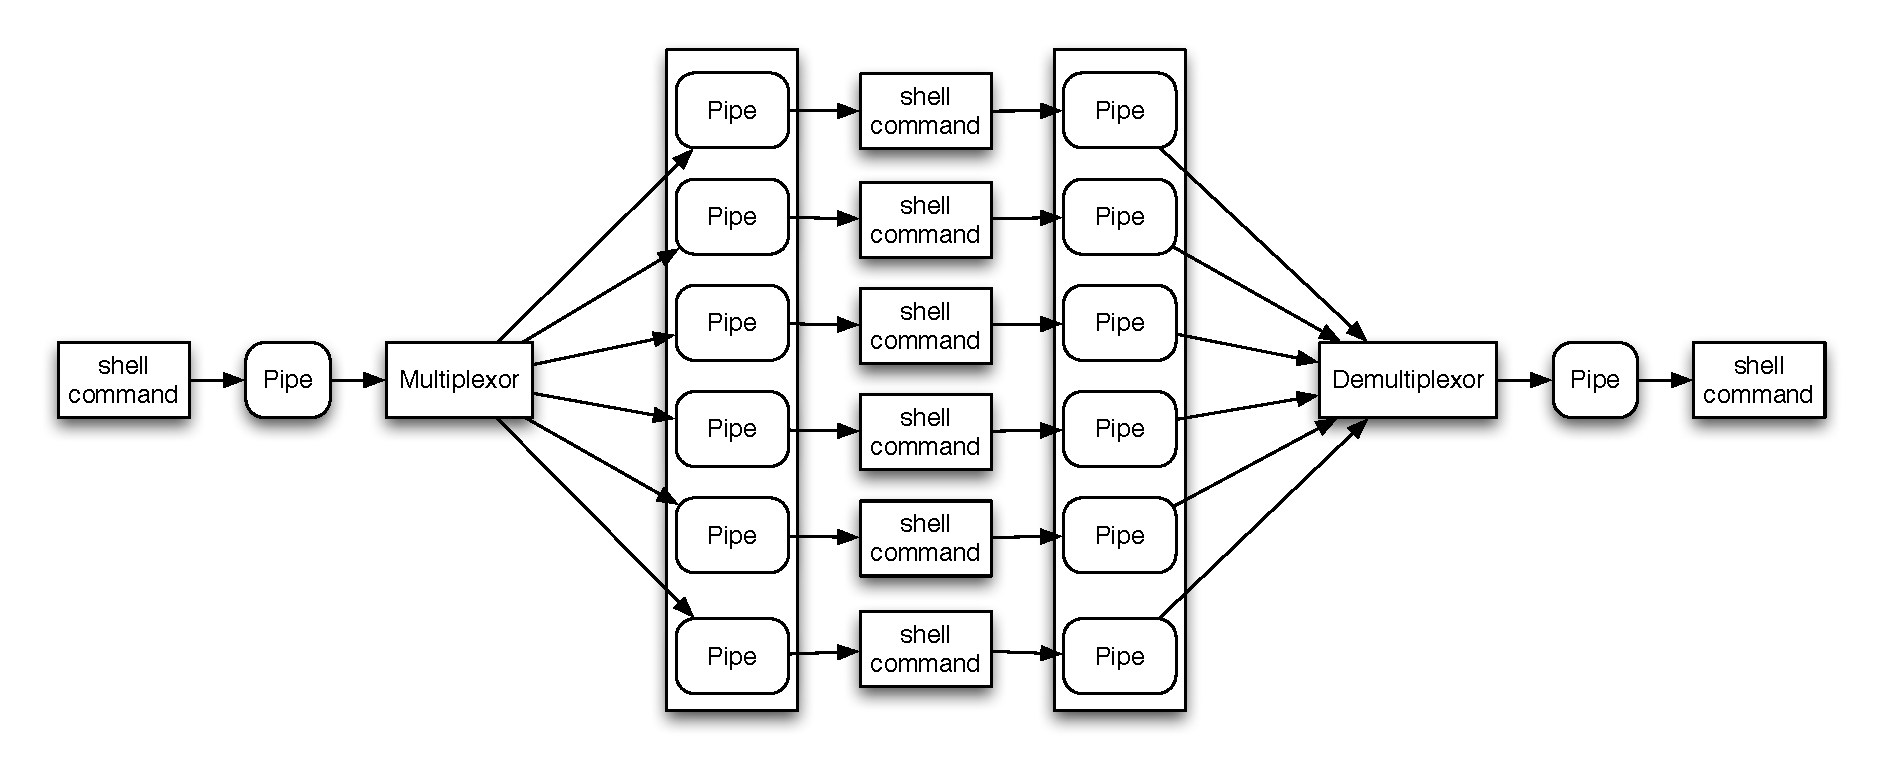
\includegraphics[width=3in]{pipestruct.eps}
\caption{The structure of the PUSH shell}
\label{fig:pipestruct}
\end{figure}

We have added two additional pipeline operators to a traditional UNIX shell,
a multiplexing fan-out(\verb!|<![\emph{n}]), and a coalescing fan-in(\verb!>|!).
 
This combination allows PUSH to distribute I/O to and from multiple
simultaneous threads of control.
The fan-out argument \emph{n} specifies the desired degree of parallel
threading.  If no argument is specified, the default of spawning a new
thread per record (up to the limit of available cores) is used.  This can
also be overriden by command line options or environment variables.
The pipeline operators provide implicit grouping semantics allowing natural
nesting and composibility.
While their complimentary nature usually lead to symmetric
mappings (where the number of fan-outs equal the number of fan-ins), there is
nothing within our implementation which enforces it.
Normal redirections as well as application specific sources and sinks
can provide alternate data paths.
Remote thread distribution and interconnect are composed and managed
using synthetic file systems in much the same manner as Xcpu,\cite{xcpu}
pushing the distributed complexity into the middleware in an language and
runtime neutral fashion.

PUSH also differs from traditional shells by implementing native support for
record based input handling over pipelines. This facility is similar to the
argument field separators, IFS and OFS, in traditional shells which use a
pattern to determine how to tokenize arguments. PUSH provides two variables,
ORS and IRS, which point to record separator modules. These modules
(called multiplexors in PUSH) split data on record boundaries, emitting
individual records that the system distributes and coalesces.

The choice of which \emph{multipipe}, an ordered set of pipes, to target is
left as a decision to the module.
Different data formats may have different output requirements.Demultiplexing from a multipipe is performed by creating a many to one
communications channel within the shell. The shell creates a reader processes
which connects to each pipe in the multipipe. When the data reaches an
appropriate record boundary a buffer is passed from the reader to the shell
which then writes each record buffer to the output pipeline.

An example from our particular experience, Natural Language Processing, is
to apply an analyzer to a large set of files, a "corpus". User programs go
through each file which contain a list of sentences, one sentence per line.
They then tokenize the sentence into words, finding the part of speech and
morphology of the words that make up the sentence.
This sort of task maps very well to the DISC model. There are a large number of
discrete sets of data whose order is not necessarily important. We need to
perform a computationally intensive task on each of the sentences, which are
small, discrete records and ideal target for parallelization.

PUSH was designed to exploit this mapping. For example, to get a histogram of
the distribution of Japanese words from a set of documents using chasen,
a Japanese morphological analyzer, we take a set of files containing sentences
and then distribute them to a cluster of machines on our network. The command
is as follows:
\begin{verbatim}
push -c '{
  ORS=./blm.dis  du -an files |< xargs os \\
   chasen | awk '{print \$1}' | sort | uniq -c \\
   >| sort -rn
}'
\end{verbatim}

The first variable, ORS, declares our record multiplexor module, the intermediar
y
used to ensure that the input and output to distributed pipes are correctly
aligned to record boundaries. du -n gives a list of the files (note that our
du is a bit different from the canonical UNIX du, it replaces much of find's
functionality) which are then "fanned out"(\verb!|<!) using a combination
of a multipipes, and a \emph{multiplexor}
which determines which pipes are the targets of each unit of output.
This fanned out data goes to xargs on other machines which
then uses the filenames(sent from the instantiating machine) as arguments to
chasen. The du acts as a command driver, fanning out file names to the
individual worker machines. The workers then use the filenames input to
xargs, which uses the input filenames as arguments to xargs target command.
Using the output of the analyzer awk extracts the first line fields(Japanese
words) which are then sorted and counted using uniq.  Finally these word
counts are "fanned in"(\verb!>|!) to the originating machine which then
sorts them.


\subsection{Aggregation Infrastructure}

\subsection{Multi-Participant Pipelining}

